%!TEX root = paper.tex
%
% GeoClaw
%
% Lead currently:  Randy LeVeque
%

\subsection{\geoclaw}

The \geoclaw branch of \clawpack was developed to solve the
two-dimensional shallow water equations over topography
for modeling tsunami generation, propagation, and inundation.
The \amrclaw code formed the starting point but it was necessary to make many
modifications to support the requirements of this application, as described
briefly below.  This code originated with the work of George
\cite{dgeorge:masters, dgeorge:phd, dgeorge:jcp}
and was initially called
{\sc TsunamiClaw}.  Later it became clear that many other
geophysical flow applications have similar requirements and the code was
generalized as \geoclaw.


One of the major issues is the treatment of wetting and
drying of grid cells at the margins of the flow. The handling of dry
states in a Riemann solver is difficult to handle robustly, and has gone
through several iterations.
\geoclaw must also be well-balanced in order to preserve steady states.
This is necessary for  waves with amplitudes that
are very small relative to the depth of the ocean to be  well-resolved.
Numerical methods that are well-balanced treat
the topography, which appears as a source term in the
momentum equations, in the Riemann solver rather than treating it as a
source term using a splitting method. \alert{Is true generally, or only in Clawpack?}
This is all incorporated into the Riemann solver developed in
\cite{dgeorge:phd, dgeorge:jcp}. Other features of
\geoclaw include the ability to solve the equations in latitude--longitude
coordinates on the surface of the sphere, and the incorporation of source terms
modeling bottom friction using a Manning formulation. More details about the
code and tsunami modeling applications can be found in
\cite{BergerGeorgeLeVequeMandli:awr11, LeVequeGeorgeBerger:an11}. In 2011, a
significant effort took place to verify and validate \geoclaw against the US
National Tsunami Hazard Mitigation Program (NTHMP) benchmarks
\cite{GonzalezLeVequeEtAl2011}.
NTHMP approval of the code allows \geoclaw to be used in hazard mapping
projects that are funded by this program or other federal and state agencies,
e.g.
\cite{GonzalezLeVequeEtAl2013a,GonzalezLeVequeEtAl2014}.
This is illustrated in \cref{fig:ocosta}.

In addition to a variety of tsunami modeling applications,
\geoclaw has been used to solve dam break problems in steep terrain
\cite{George:Malpasset}, storm surge problems \cite{Mandli:ws} (see \cref
{fig:surge}),
and submarine landslides \cite{jhkim:phd}.  The code also
formed the basis for solving the
multi-layer shallow water equations for storm surge modeling
\cite{mandli:phd, Mandli:2013it},
and is currently being extended further to handle debris flow modeling in the
packages D-Claw
\cite{Iverson:2014dc,George:2014gh} (see Figure~\ref{fig:meager}).

Roughly one third of the files in the \amrclaw source library have to be
modified for \geoclaw. There are currently 135 files in the \amrclaw 2D branch.
Forty-five of them are replaced by a \geoclaw-specific file of the same name but
in the \geoclaw 2D branch. For example, to keep a flat sea level when
interpolating, it is necessary to account for topography. This implies that the
water height plus topography is interpolated rather than just interpolating the
conserved quantity, which is the default behavior in
\amrclaw.

Several other substantial improvements in the
algorithms implemented in \geoclaw have been made between versions 4.6 and
5.3.0, including:

\begin{itemize}
\item In depth-averaged flow, the wave speed and therefore the CFL
condition depends on the depth.  As a result, flows in shallow water
that have been refined spatially may not need to be refined in time.
This ``variable-time-stepping'' was easily added along with the anisotropic
capabilities that were added to \amrclaw.
\item The ability to specify topography via a set of {\tt
topo} files that may cover overlapping regions at different resolutions has been added.
 The finite volume method requires cell averages of topography, computed by
integrating a piecewise bilinear function constructed from the input {\tt
topo} files over each grid cell.  In \clawpack 5.1.0, this was improved to
allow an arbitrary number of nested {\tt topo} grids.
When adaptive mesh refinement is used,
regridding may take place every few time steps.  Improvements were made
in 5.2.0 so that topography could be copied rather than always being
recomputed in regions where there is an existing old grid.

\item The user can now provide multiple  {\tt dtopo} files that
specify changes to the
initial topography at a series of times.  This is used to specify sea-floor
motion during a tsunamigenic earthquake, but can also be used to specify
submarine landslide motion or a failing dam, for example.
%Major changes were
%made to these algorithms in 5.1.0 to fix a problem in earlier versions that
%resulted in incorrect topography motion in some cases, also resulting in a much
%more robust handling of multiple  {\tt dtopo} files.

\item A number of new Python modules has been developed to assist the user
in working with {\tt topo} and {\tt dtopo} files.  These are documented in
the \clawpack documentation and several of them are illustrated with Jupyter
notebooks found in the \clawpack Gallery.

\item New capabilities were added in 5.0.0 to monitor the maximum of
various flow quantities over a specified time range of a simulation.
This capability is crucial for many applications where the maximum
flow depth at each point, maximum current velocities in a harbor, or
maximum momentum flux (a measure of the hydrodynamic force that would
be exerted by the flow on a structure) is desired.  Arrival time of
the first wave at each point can also be monitored.  Such
capabilities were included in the 4.x version of the code, but were
more limited and did not always perform properly near the edges of
refinement patches.  In Version 5.2 these routines were further
improved and extended.  The user can specify a grid of points on which
to monitor values, and the new code is more flexible in allowing
one-dimensional grids (e.g. a transect), two-dimensional rectangular
grids, or an arbitrary set of points.  This is described in
\url{http://www.clawpack.org/fgmax.html}.

\end{itemize}

\begin{figure}
\hfil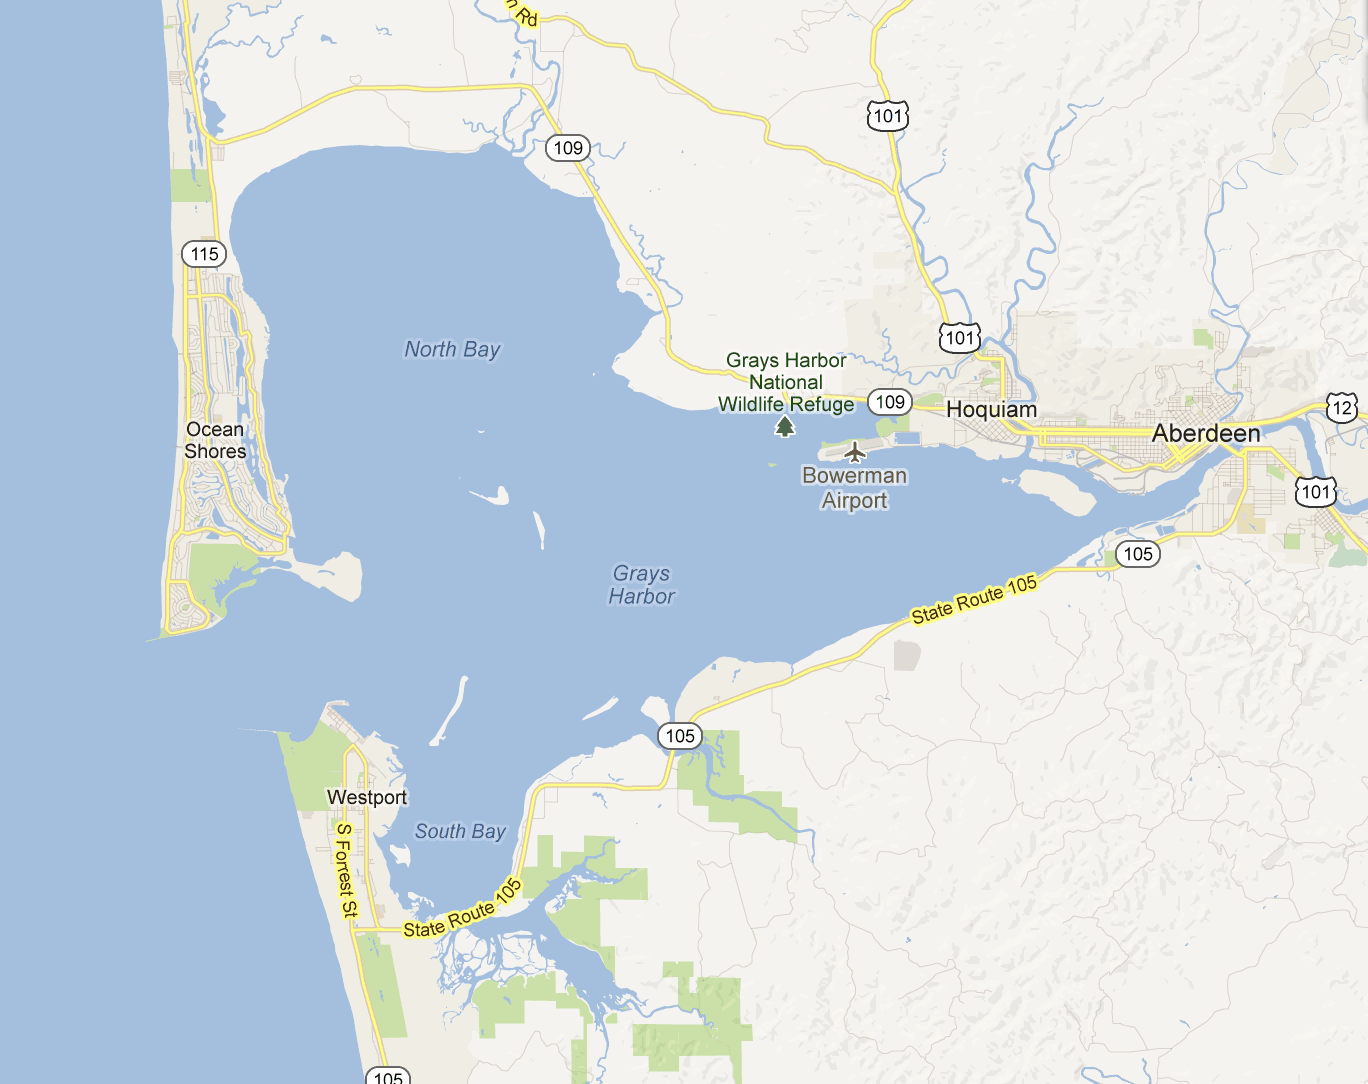
\includegraphics[height=1.2in]{Grays.png}
\hskip 5pt
\hfil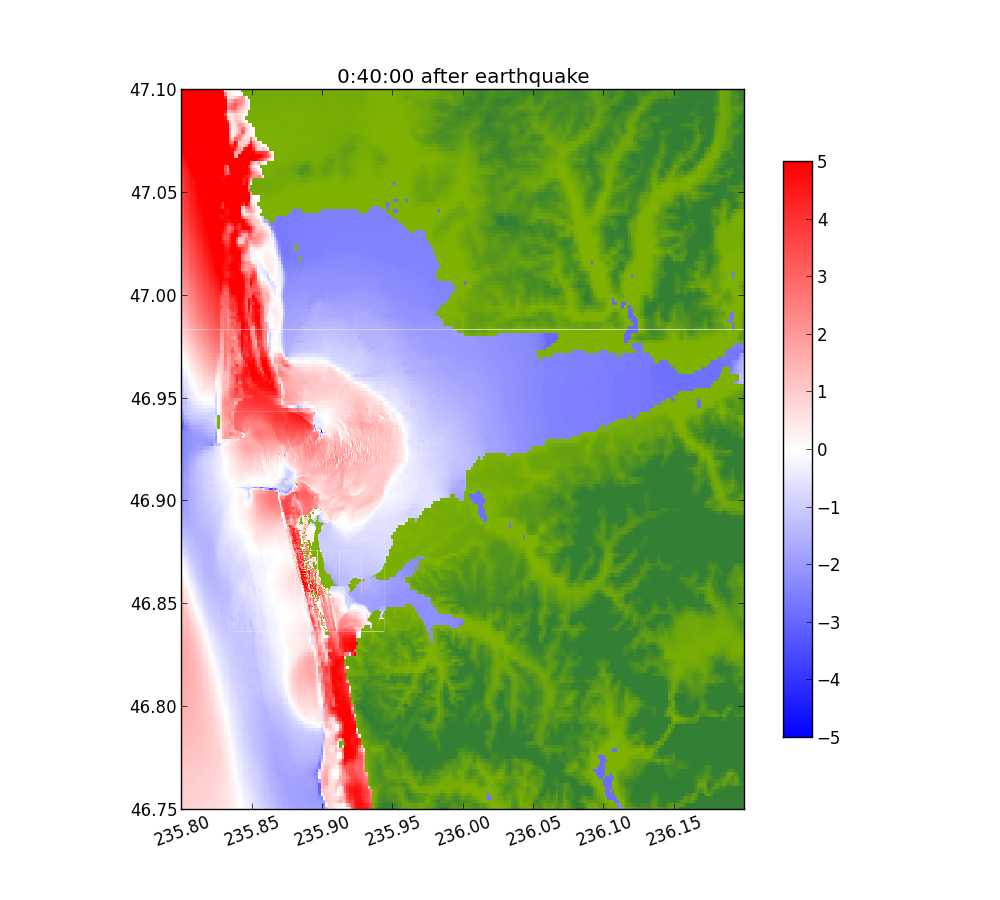
\includegraphics[height=1.4in]{GraysHarbor40.png}
\hskip 5pt
\hfil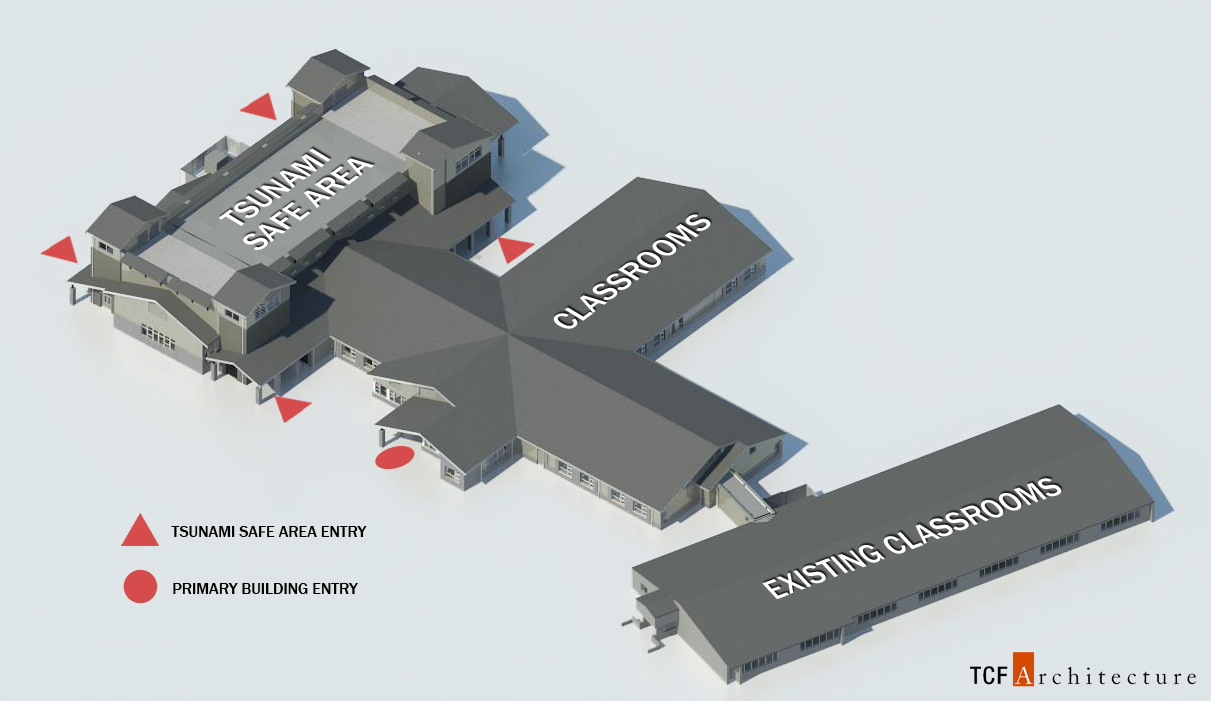
\includegraphics[height=1.2in]{OcostaExteriorRendering_2014-5-15.jpg}
\hskip 5pt
\caption{\label{fig:ocosta}
Left: Gray's Harbor showing Westport, WA on southern peninsula.
Middle: Simulation of a potential magnitude 9
Cascadia Subduction Zone event, 40 minutes after the earthquake.
Right: Design for new Ocosta Elementary School in Westport, based in part on
\geoclaw simulations \cite{GonzalezLeVequeEtAl2013a}.
  }
\end{figure}

\begin{figure}[t]
    \centering
    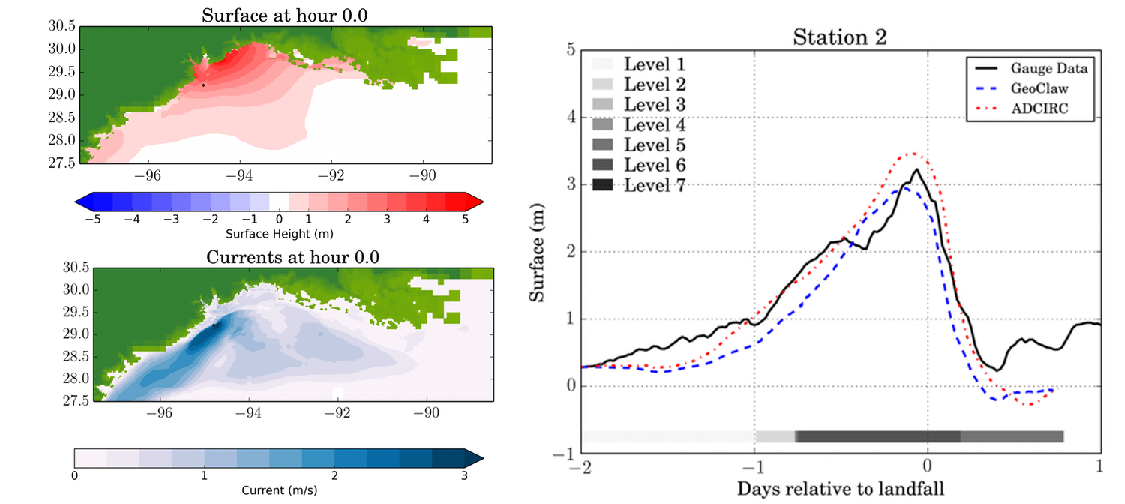
\includegraphics[width=\textwidth]{surge_figure}
\vskip 5pt
    \begin{tabular}{|c|c|c|c|}
        \hline
        {\bf Package} & {\bf Threads} & {\bf Wall Time} & {\bf Core Time} \\
        \hline
        {\sc ADCIRC} & 4000 & 35 minutes & 2333 hours \\
        \geoclaw & 4 & 2 hours & 8 hours \\
        \hline
    \end{tabular}
    \caption{Top Left: A snapshot of a \geoclaw storm surge simulation of
Hurricane Ike at landfall.  Top Right:  Tide gauge data computed from \geoclaw
and {\sc adcirc} along with observed data at the same location.
Bottom: Computational effort and timings for \geoclaw and ADCIRC.  From
\cite{Mandli:ws}. \label{fig:surge}}
\end{figure}

\begin{figure}[t]
\hfil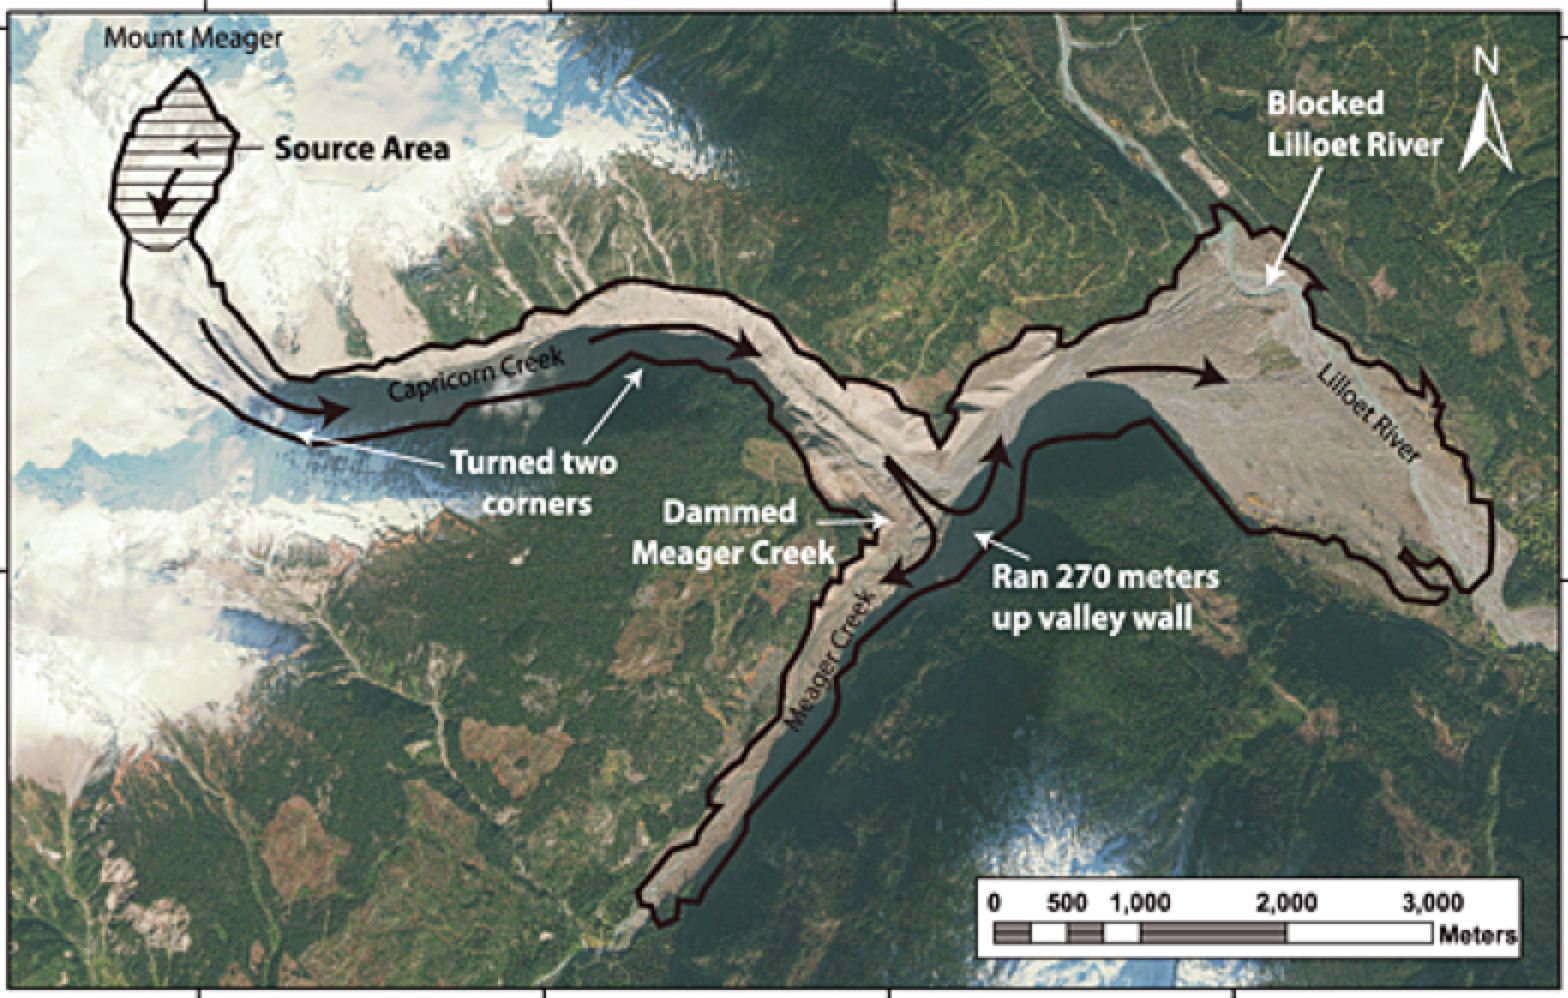
\includegraphics[height=1.3in]{meagerview.png}
\hskip 5pt
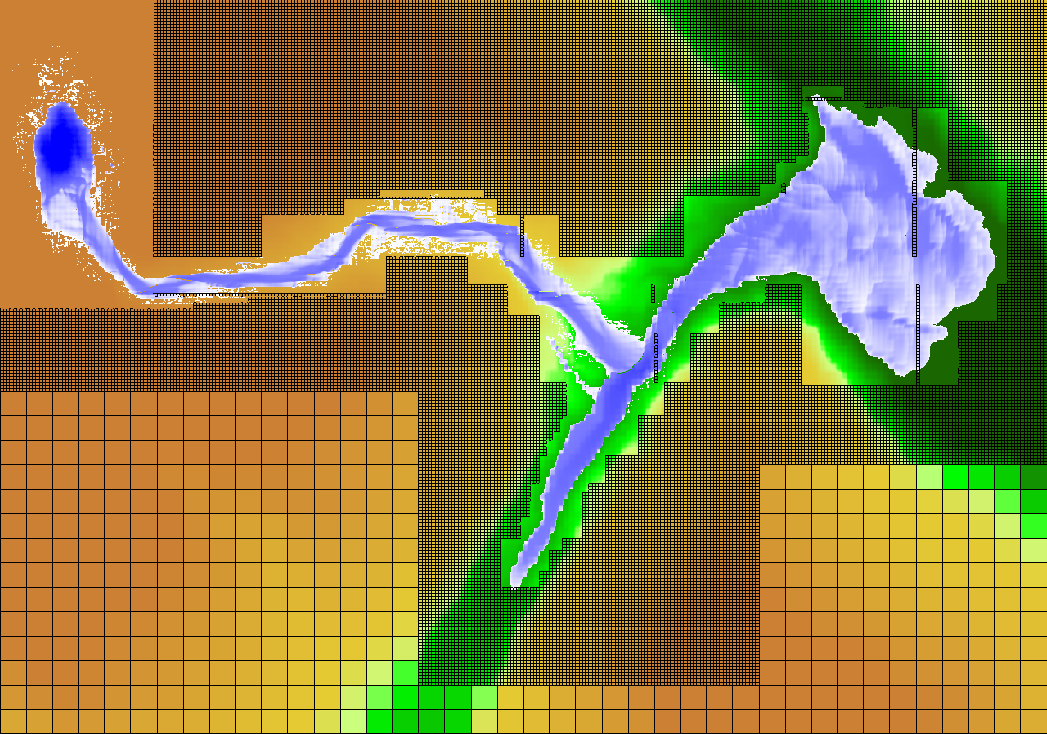
\includegraphics[height=1.3in]{meager200.png}\hfil
\hskip 5pt
\includegraphics[height=1.3in]{Oso_comparison.jpg}\hfil
\caption{\label{fig:meager}
Left: Mt.\ Meager debris flow of 2010, from \cite{Allstadt2013}.
Middle: Simulated debris flow, from D.\ George.
Right: Observed (yellow line) and computed (blue) landslide at Oso, WA in
2014 \cite{IversonGeorgeEtAl2015}.}
\end{figure}
